\documentclass{article}
\usepackage{tikz}
\begin{document}
\resizebox{!}{\textheight}{%
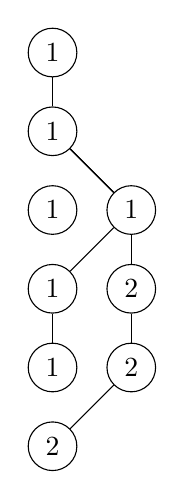
\begin{tikzpicture}[]
\node[draw, circle] (0&1) at (0,0) {1};
\node[draw, circle] (1&1) at (0,-1) {1};
\node[draw, circle] (2&1) at (0,-2) {1};
\node[draw, circle] (2&1) at (1,-2) {1};
\node[draw, circle] (3&1) at (0,-3) {1};
\node[draw, circle] (3&2) at (1,-3) {2};
\node[draw, circle] (4&1) at (0,-4) {1};
\node[draw, circle] (4&2) at (1,-4) {2};
\node[draw, circle] (5&2) at (0,-5) {2};
\draw (0&1) -- (1&1);
\draw (1&1) -- (2&1);
\draw (1&1) -- (2&1);
\draw (2&1) -- (3&1);
\draw (2&1) -- (3&2);
\draw (3&1) -- (4&1);
\draw (3&2) -- (4&2);
\draw (4&2) -- (5&2);
\end{tikzpicture}%
}
\end{document}
